\documentclass[12pt]{article}

\usepackage{sbc-template}
\usepackage{graphicx,url}
\usepackage[utf8]{inputenc}
\usepackage[brazil]{babel}
\usepackage{algpseudocode}
\usepackage[Algoritmo]{algorithm}
\usepackage{textgreek}
\usepackage{float}

%\usepackage[latin1]{inputenc}  

     
\sloppy

\title{BSN - Uma proposta para reduzir a latência em Redes ópticas para \emph{Smart Grid} e \emph{Smart Cities}}

\author{Daniel A. Oleinik\inst{1}, Mauro S. Fonseca\inst{1}, Anelise Munaretto\inst{1}}


\address{CPGEI -- Universidade Tecnológica Federal do Paraná (UTFPR)\\
  CEP 80.230-910 -- Curitiba -- PR -- Brasil
%\nextinstitute
  %CPGEI -- Universidade Tecnológica Federal do Paraná (UTFPR)\\
  %CEP 80.230-910 -- Curitiba -- PR -- Brasil
%\nextinstitute
  %CPGEI -- Universidade Tecnológica Federal do Paraná (UTFPR)\\
  %CEP 80.230-910 -- Curitiba -- PR -- Brasil
  \email{daniel.oleinik@outlook.com, maurofonseca@utfpr.edu.br, anelise@utfpr.edu.br }
}

\begin{document} 

\maketitle

\begin{abstract}
  The increasing consumption of energy from nonrenewable and finite sources is encouraging the advance of development and use
of new energy generation options. These options, when incorporated into the current electricity generation and distribution system,
should demand new requirements from the communication system used to provide the communication link between the network
equipment used, motivating the development of Smart grid. This document proposes a method to improve and optimize the network/access grid, built with optic fiber and mesh topology. This improvement is achieved by the handling of the physical connections in the network together witha smart reactive management, using a set of optical switches and a control software with genetic algorithm.
\end{abstract}
     
\begin{resumo} 
 O crescente consumo de energia proveniente de fontes não renováveis e finitas vem incentivando o avanço no desenvolvimento e utilização de novas opções de geração de energia. Estas opções, quando incorporadas ao sistema atual de geração e distribuição de energia elétrica, devem demandar novas exigências do sistema de comunicação utilizado entre os equipamentos da rede, motivando o desenvolvimento do \emph{Smart Grid} (SG). O presente documento propõe um método para melhoria e otimização de uma rede/\emph{grid} de acesso construída em fibra óptica com topologia \emph{mesh}. Esta melhoria é realizada através de alterações das conexões físicas da rede, em conjunto com uma gerência reativa inteligente, utilizando um conjunto de chaveadores ópticos atrelados a um software com algoritmo genético.
\end{resumo}


\section{Introdução}

A utilização de combustíveis fósseis, o aquecimento global e o aumento da população mundial, que reflete-se no aumento na demanda por energia, têm se tornado tópicos cada vez mais importantes no cenário global. Estes fatos têm acelerado o desenvolvimento de fontes renováveis de energia, como a eólica ou solar, que prometem causar menos impactos ambientais do que as principais fontes usadas atualmente. A integração dessas novas fontes de energia aos sistemas existentes de distribuição e transmissão, demanda a existência de um novo \emph{grid} de comunicação que ofereça uma infraestrutura mais rápida, eficiente e confiável do que o \emph{grid} atual \cite{Art_Gungor2013}.

Ainda segundo \cite{Art_Gungor2013}, as tecnologias de energia renovável possuem certa tendência natural de instalação não centralizada. Exemplos disso são, os geradores que se utilizam de células fotovoltaicas ou os geradores eólicos, já que ambos aproveitam-se de características geográficas e/ou climáticas. Logo, a inserção destas tecnologias deve transformar o sistema de distribuição atual em um grande sistema de geração distribuída de energia, tornando-se dessa forma, imperativo a utilização de uma infraestrutura capaz de suprir as necessidades de comunicação demandadas pela variedade de sensores, atuadores e elementos utilizados no controle desta nova rede de geração e distribuição de energia. O que, em resumo, representa o próprio conceito de \emph{Smart Grid} (SG).

Este conceito de infraestrutura refere-se a uma completa modernização no sistema de energia visando monitorar, proteger e otimizar a operação dos elementos utilizados na rede. Englobam-se aqui os elementos desde os mais básicos como os presentes em residências e utilizados por consumidores finais, até os mais críticos como os elementos geradores/armazenadores de energia ou aqueles presentes nas redes de alta tensão \cite{Conf_Sood2009}.

Neste novo cenário de Geração Distribuída de energia (DG - \emph{Distributed Generation}) pode-se observar que a ligação entre os diversos equipamentos utilizados, tanto na geração quanto na distribuição de energia, naturalmente segue uma topologia de malha ou \emph{mesh}. Isto viabiliza a aplicação de novos métodos na análise e resolução de problemas na rede de distribuição e na segurança/estabilidade da mesma, como a utilização de \emph{Self Healing} por exemplo \cite{Art_Amin2006}. Mas para isso, além da existência de uma rede de comunicação inteligente ou \emph{Smart Grid}, também faz-se necessário o atendimento de requisitos específicos de comunicação \cite{Conf_Sood2009}.

O SG necessita de grande flexibilidade para permitir a adição de serviços cada vez mais variados e com diferentes requisitos de comunicação, como monitoramento de sensores em tempo real e interação com atuadores e usuários finais \cite{Art_Aggarwal2010}. Sabe-se que uma rede IP deve atender, com elevado grau de satisfação, os requisitos de comunicação demandados \cite{Conf_Lobo2008}. Requisitos estes que, segundo \cite{Art_Aggarwal2010}, devem ser substancialmente consideráveis tanto em largura de banda quanto em valores de latência, justificando facilmente o uso de um meio físico como a fibra óptica assim como qualquer tentativa de redução de latência. O presente documento vai de encontro a esta demanda, visto que propõe um método de redução de latência, baseado na diminuição do número de saltos entre a origem e o destino da comunicação em uma rede IP, através da utilização de chaveadores ópticos estrategicamente acionados por um software com algoritmo genético.

\section{Conceitos Básicos}

A presente seção destina-se a uma breve explicação sobre alguns dos conceitos utilizados neste documento. Sendo que, naturalmente, nenhum dos conceitos aqui apresentados será abordado de maneira extensiva.

\subsection{PRIM}
\label{subsec:Prim}
O algoritmo PRIM é recorrentemente utilizado por muitos outros algoritmos para encontrar a árvore geradora mínima de um grafo completamente conectado. Este algoritmo foi criado em 1930 por um matemático Tchecoslovaco chamado Vojtěch Jarník, melhorado em 1957 por um matemático e cientista da computação americano chamado Robert Clay Prim (que acabou dando nome ao algoritmo) e posteriormente utilizado em 1959 por Edsger Dijkstra (responsável pela criação do Algoritmo de Dijkstra).

Este algoritmo considera uma subárvore do grafo em questão e a expande, observando o critério da minimalidade baseada em cortes, até que ela se torne a árvore geradora mínima (MST - \emph{Minimal Spanning Tree} do mesmo. O algoritmo pode ser aplicado a qualquer grafo conexo não direcionado e não leva em consideração a utilização de um nó origem.

\subsection{STP - \emph{Spanning Tree Protocol}}
\label{subsec:STP}
O protocolo STP, definido no IEEE 802.1D, é comumente utilizado por \emph{switches} para evitar \emph{loops} em \emph{layer} 2. Os \emph{switches} de uma rede STP comunicam-se e descobrem a topologia geral da rede, para então desligar ou bloquear as portas dos equipamentos onde existam \emph{loops} \cite{Art_Krishnan}.

Os estados possíveis das portas dos equipamentos utilizadas no protocolo STP podem ser: \emph{Blocking, Listening, Learning, Forwarding} ou \emph{Disabled} \cite{Art_Wojdak}. Dessa forma, o protocolo pode garantir que as conexões que causam os \emph{loops} existentes na rede possam deixar de ser utilizadas, mantendo-as como possíveis opções de conexão caso a principal seja perdida.

Este protocolo considera um equipamento da rede como sendo o nó raiz e a partir dele a topologia resultante de rede pode ser obtida ao mesmo tempo que os \emph{loops} são evitados (sendo transformados em rotas alternativas em caso de falha). Como este protocolo é padrão e amplamente difundido, ele também é o protocolo mais utilizado em redes SG reais.

\subsection{Chaveador ótico}
Apesar das visíveis diferenças entre cabos elétricos e ópticos, pode-se fazer um paralelo entre os dois de maneira satisfatória caso suas particularidades sejam devidamente respeitadas. 

Considerando-se que a transmissão de informação dentro de uma fibra óptica é realizada através da condução da luz dentro do núcleo da mesma, através do fenômeno de Reflexão Interna Total (fenômeno originado na diferença do índice de refração entre o material utilizado
na fabricação do núcleo da fibra e o utilizado em sua capa envoltória protetora, também chamada de casca \cite{inbook_data_cabling}) conforme representado na Figura \ref{fig_fibra_optica} e considerando  também que a fibra óptica funciona como um guia para a luz, pode-se entender que uma fibra óptica, sob circunstâncias controladas (alinhamento, proximidade e características de núcleo), pode enviar sinais a outra fibra. 

\begin{figure} % normalmente utilizar [!t]
	\centering
	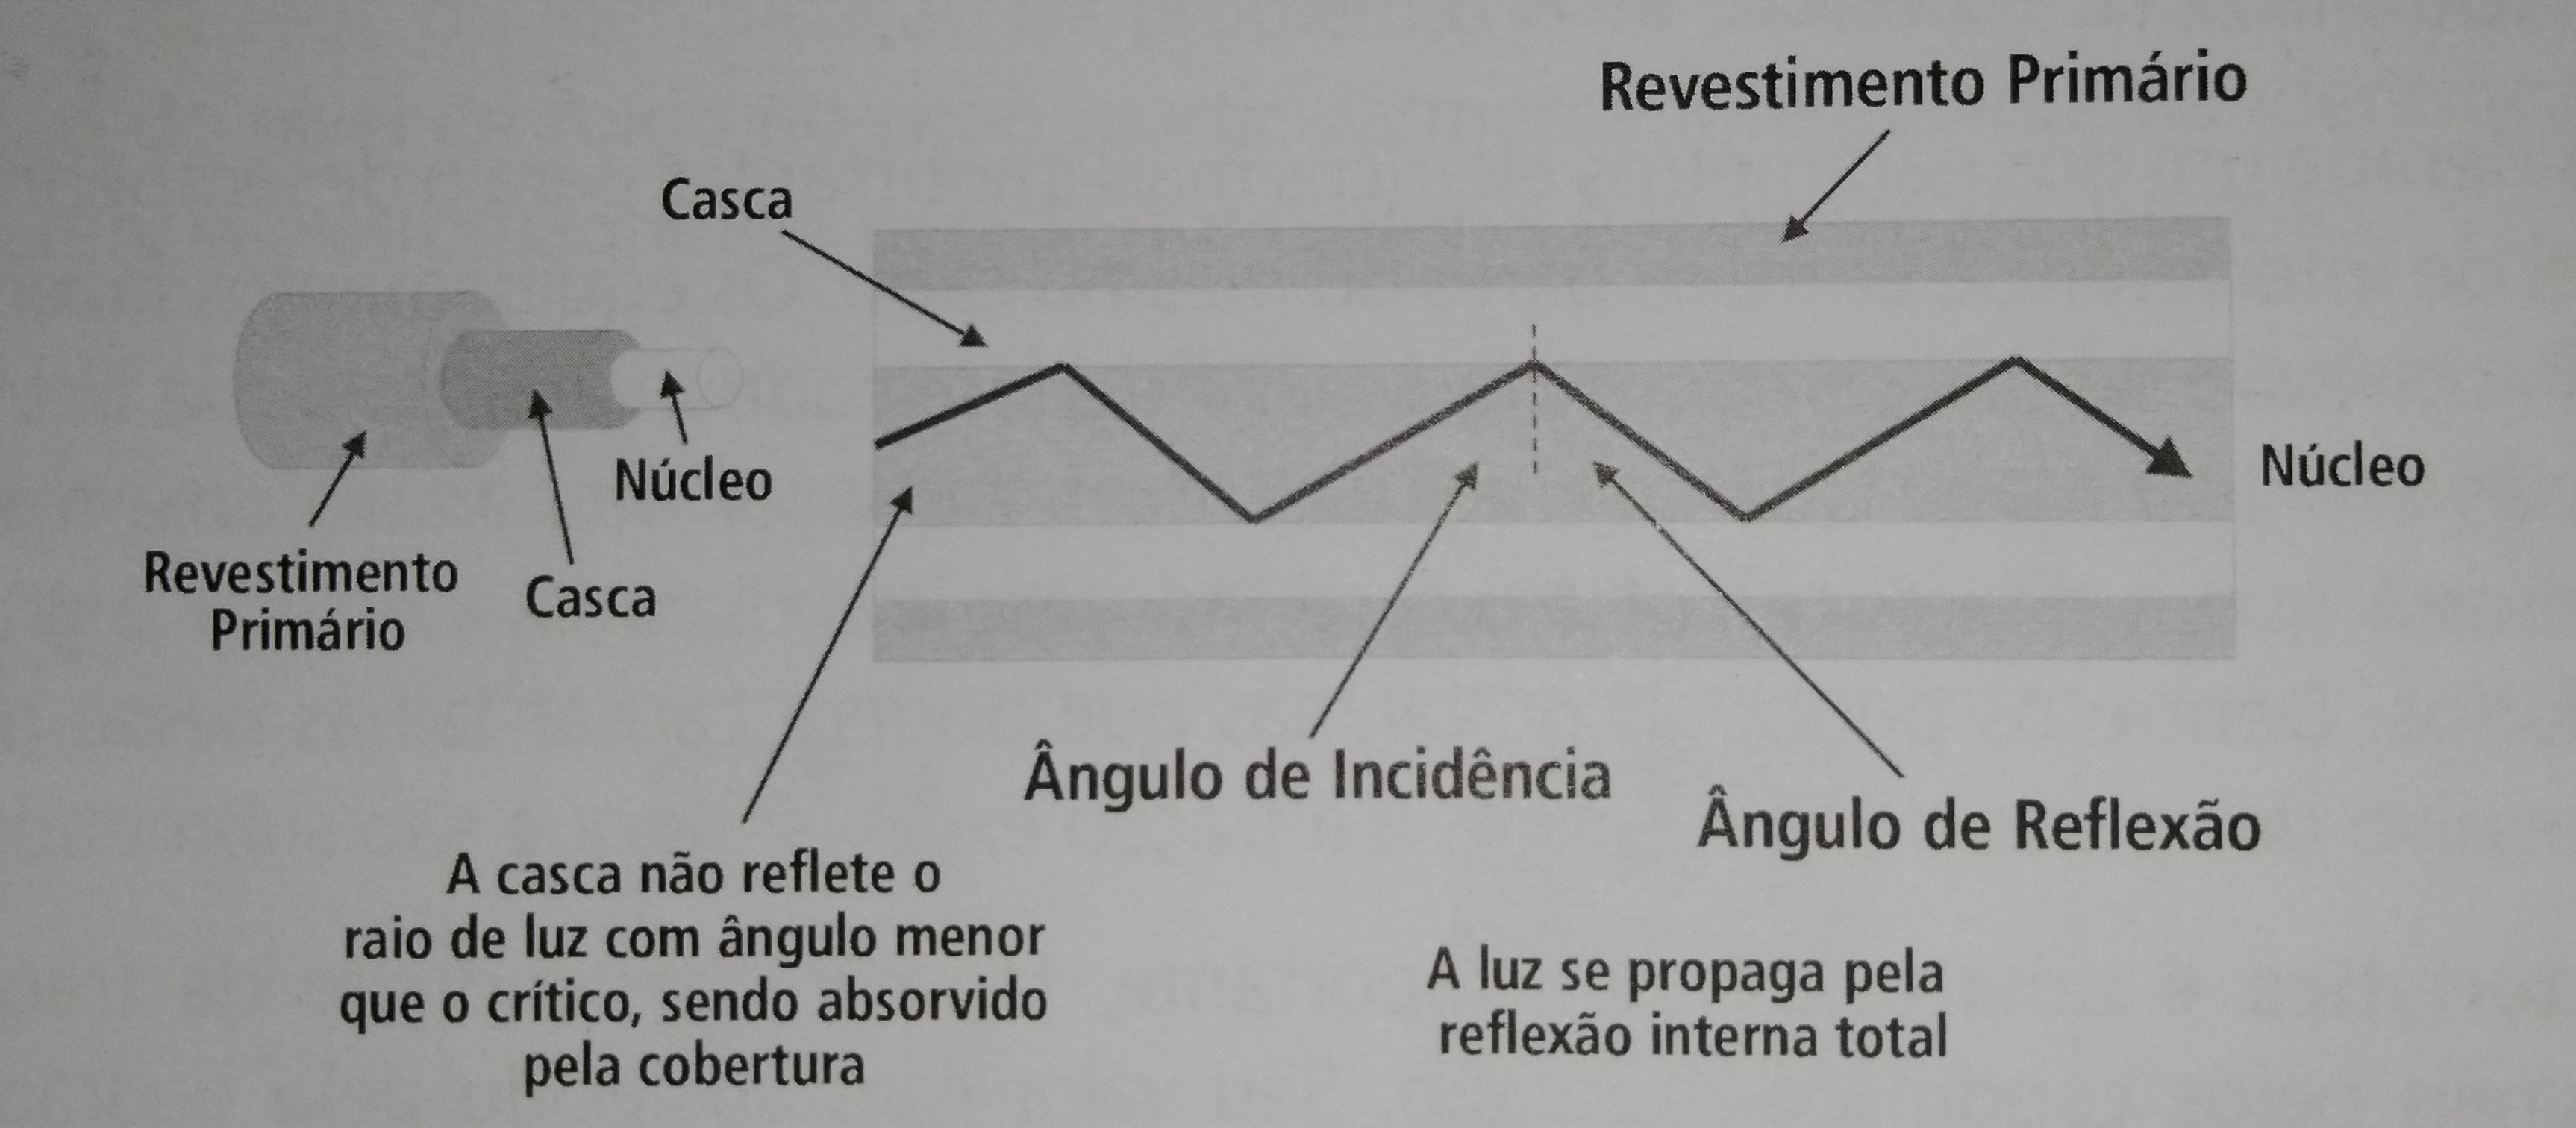
\includegraphics[width=8cm]{fibra_optica}
	\caption{Representação do fenômeno de reflexão interna total em uma fibra óptica. Fonte: \cite{inbook_data_cabling}}
	\label{fig_fibra_optica}
\end{figure}

\begin{figure} [h]% normalmente utilizar [!t]
	\centering
	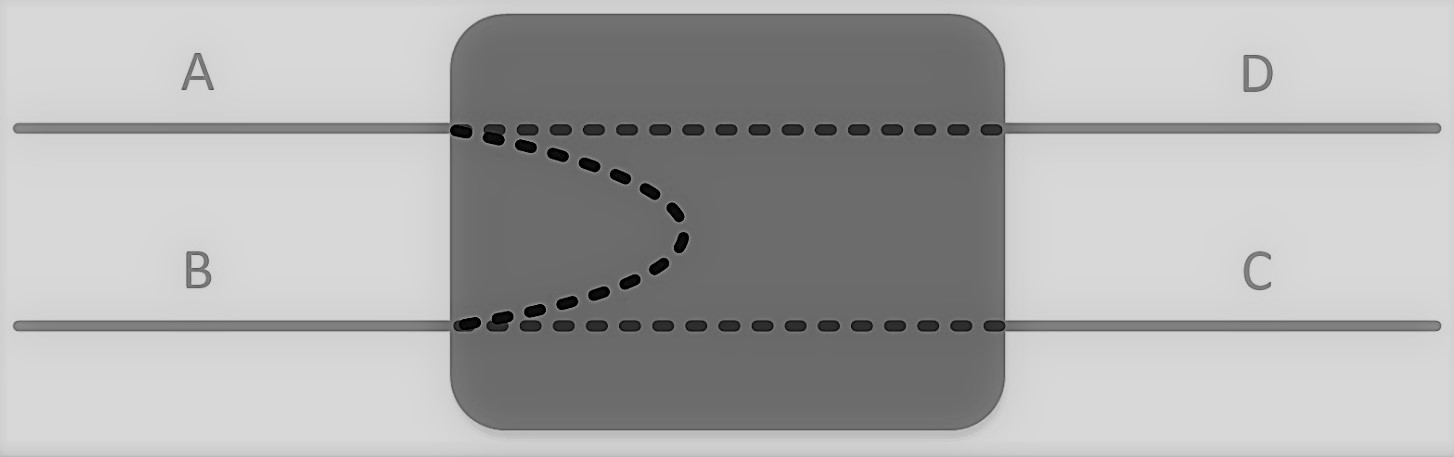
\includegraphics[width=7cm]{Switch_optico}
	\caption{Diagrama interno simplificado de um chaveador óptico. Em um estado este componente transmite bidirecionalmente a luz da interface A para D e B para C, quando acionado ele transmite bidirecionalmente a luz da interface A para B. Adaptado de \cite{Accelink2014}}
	\label{fig_switch_optico}
\end{figure}

Desse modo, pode-se imaginar a construção de um relé óptico onde, analogamente a um relé metálico, as fibras de entrada e saída são chaveadas de acordo com um sinal de entrada. Tal equipamento recebe o nome neste documento de chaveador óptico e é representado simplificadamente na Figura \ref{fig_switch_optico}. 

Existem diversos modelos de chaveadores ópticos presentes no mercado, sendo que todos eles baseiam-se no mesmo princípio de funcionamento. Eles são capazes de encaminhar a luz de uma entrada à outra através de um prisma acoplado à uma bobina elétrica, desta forma a posição do prisma pode ser manipulada para realizar a conexão entre diferentes entradas e saídas.

\subsection{Topologia \emph{Mesh}}
Este tipo de topologia, também chamada de topologia em Malha, é muito comum em diversas aplicações como as Industriais, IoT, comunicações em longas distâncias, sem fio ou em meios complexos de maneira geral. 

Esta topologia adapata-se bem a estes cenários visto que uma das grandes vantagens deste tipo de tecnologia é a quantidade de rotas redundantes que ela oferece. Isto deve-se ao fato de que cada nó comunica-se com todos os presentes em seu alcance e cada um deles tem a capacidade de repetir mensagens até que a mesma alcance seu destino. 

Esta topologia de rede poder ser implementada independentemente do meio físico utilizado, a Figura \ref{fig_rede_mesh} ilustra uma rede \emph{Mesh} cabeada, visto que este tipo de rede será alvo do estudo realizado no presente documento.

\begin{figure} % normalmente utilizar [!t]
	\centering
	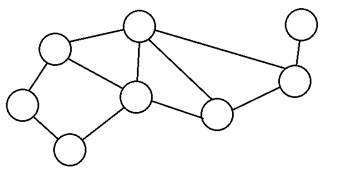
\includegraphics[width=5cm]{Rede_Mesh}
	\caption{Exemplo de uma rede cabeada em topologia \emph{Mesh}. Nota-se que os vizinhos de cada nó estão fisicamente interconectados e que nem todos os nós alcançam diretamente uns aos outros (é necessário retransmissão de pacotes por parte dos nós intermediários para estabelecer a comunicação).}
	\label{fig_rede_mesh}
\end{figure}

\section{Cenário de Estudo}
\label{sec:Ambientacao}
Tipicamente existem dois cenários em aplicações SG para distribuição de energia elétrica: um ambiente rural pouco populado ou um ambiente urbano densamente populado e naturalmente conectado em \emph{grid} \cite{Conf_Sood2009}. Este último tipo de conexão é muito útil por possibilitar a manobra da rede elétrica, através da utilização de chaves específicas, para garantir a utilização de sensores e atuadores diversos além de possibilitar o fornecimento de energia ao máximo número possível de consumidores sob circunstâncias de falhas. A Figura \ref{fig_rede_distribuicao} exemplifica este tipo de ligação.

\begin{figure} % normalmente utilizar [!t]
	\centering
	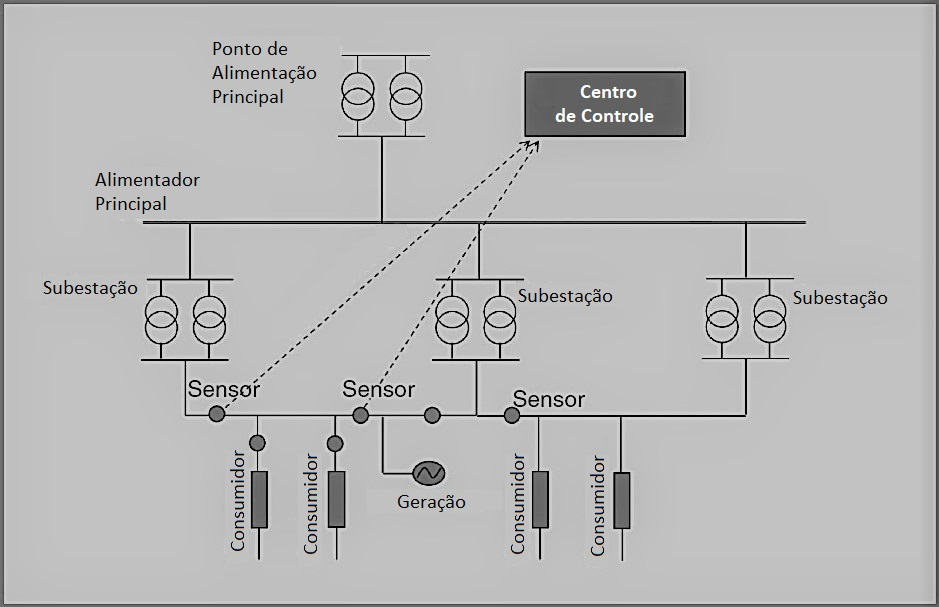
\includegraphics[width=7cm]{Rede_Distribuicao}
	\caption{Exemplo de uma rede de distribuição de energia elétrica conectada em malha. Esta conexão possibilita o redirecionamento de energia para os consumidores em caso de falha em um dos circuitos ou subestações. Adaptado de \cite{Mag_Bouhafs2012}}
	\label{fig_rede_distribuicao}
\end{figure}

O conceito de SG engloba diversos tipos de serviços, que devem coexistir em uma rede de comunicação de maneira satisfatória visando garantir a correta operação do sistema. Logo, é normal que existam diversas exigências de funcionamento e desempenho. Segundo \cite{Art_Aggarwal2010} pode-se prever nessa rede um elevado número de mensagens devido ao grande número de elementos adicionados à rede. Essas mensagens devem crescer muito mais rapidamente que o número de elementos, visto que deve-se extrair várias informações de cada um deles. Também são esperados elevados requisitos de desempenho com relação à latência, visto que todas essas mensagens devem ser enviadas a um centro de controle, que será o responsável pela análise dos dados recebidos para tomada de decisão. Por isso, caso alguma das mensagens sofra grande latência, ela poderá chegar ao seu destino atrasada demais para a tomada de decisão, como o acionamento de uma chave de alta tensão por exemplo, conduzindo o sistema a resultados errôneos.

Outro requisito de grande importância, é a confiabilidade do sistema de comunicação utilizado para estabelecer a rede de SG. Um dos cenários mais exigentes deste quesito origina-se nas fontes renováveis de energia. É fácil perceber que elementos como geradores fotoelétricos ou eólicos são intrinsecamente dependentes de condições externas como nível de insolação local ou quantidade e velocidade dos ventos. Logo eles não são capazes de gerar uma quantidade constante de energia, por isso os dispositivos de armazenamento representam um ponto importante no sistema. Eles devem ser responsáveis por possibilitar o armazenamento da energia gerada para posterior uso em momentos de baixa produção. Mas para isso é necessária uma alta disponibilidade da rede, promovendo acesso instantâneo de informações de geração sob praticamente qualquer circunstância, exigindo-se níveis de confiabilidade entre 99\% e 99,99\% \cite{Art_Gungor2013}.

Considerando que, de maneira geral, o modo mais seguro de aumentar o nível de confiabilidade de um sistema de comunicação seria oferecer uma rota redundante para o mesmo, podemos dizer que quanto mais rotas redundantes forem oferecidas maior o nível de confiabilidade alcançado na rede. Neste sentido, um equipamento de comunicação que fornece a possibilidade do estabelecimento de uma rede óptica utilizando um \emph{grid} ou topologia \emph{mesh} deve, naturalmente, oferecer grande aderência às necessidades da rede.

%Redes como a descrita, são comumente encontradas em cenários de SG em DG, e normalmente são estabelecidas através da utilização de protocolos de roteamento padrão como \emph{"Spanning Tree Protocol"} (STP). O STP tem a função básica de calcular os caminhos ótimos para a comunicação entre o centro de controle da rede e os equipamentos de campo, eliminando os \emph{loops} decorrentes da ligação \emph{mesh} utilizada para o estabelecimento do \emph{grid}. Para isso o protocolo determina as rotas mais eficientes (de menor custo) em cada um dos segmentos de rede. Resultando em um grafo mínimo da rede que conecta todos os nós.
Na prática, as redes utilizadas em cenários de SG em DG, são criadas com o máximo de redundâncias possíveis controladas através da utilização de protocolos de roteamento como o STP, que neste caso, tem a função básica de calcular os caminhos ótimos para a comunicação entre o centro de controle da rede e os equipamentos de campo, eliminando os \emph{loops} decorrentes dos múltiplos caminhos existentes na topologia utilizada para o estabelecimento do \emph{grid}. Para isso o protocolo determina as rotas mais eficientes (de menor custo) em cada um dos segmentos de rede otimizando o grafo da rede e garantindo a conexão entre todos os nós.

\section{BSN - \emph{Bypass} Seletivo de Nós}
\label{sec:proposta}
O presente artigo tem como proposta o protocolo BSN, cujo objetivo é a descoberta e estabelecimento de rotas completamente desagregado do protocolo de roteamento utilizado na rede em questão. O protocolo proposto pode ser utilizado em qualquer rede que contenha multi-caminhos ou redundâncias, apesar de apresentar melhores resultados quando aplicado à redes \emph{mesh} devido a maior possibilidade de recombinações. Para tanto, é necessário que a rede em questão possa ser representada por um grafo simples, ou seja, um grafo que não possui arestas paralelas ou pontas coincidentes (laços).

De maneira geral, uma rede \emph{mesh} apresenta vários possíveis caminhos entre o ponto inicial e destino da comunicação, sendo que dessa forma existem custos atrelados ao roteamento, encaminhamento e processamento de pacotes em qualquer comunicação neste tipo de topologia. A proposta atua no refino destes custos através do estabelecimento de caminhos específicos/estratégicos para cada enlace.

Basicamente existem dois tipos de equipamentos que podem ser utilizados em redes ópticas (como as apresentadas na seção \ref{sec:Ambientacao}), os puramente ópticos e os elétricos. Os equipamentos puramente ópticos possuem custo muito elevado e são muito sensíveis, já que têm a capacidade de realizar o roteamento de luz (baseado no comprimento de onda dos sinais) e por isso não são utilizados em larga escala, normalmente esse tipo de tecnologia pode ser encontrado em alguns filtros e \emph{splitters} especiais. Já os equipamentos elétricos possuem custos muito mais atrativos e são normalmente empregados para roteamento de maneira geral, mas em contrapartida são sensivelmente mais lentos.

Os atrasos existentes em equipamentos elétricos utilizados em redes ópticas têm diversas origens, como o processamento dos dados (intrinsecamente relacionado ao poder de processamento do equipamento) e as conversões de meio necessárias, sendo que para cada equipamento pode-se considerar pelo menos duas dessas conversões (óptica-elétrica-óptica). 

Logo, todas as vezes que um pacote trafega em uma rede óptica, acaba sofrendo atrasos que são traduzidos em forma de latência, que devem ser somadas a fim de determinar a latência total de um enlace. A Figura \ref{fig_latency_link} mostra a acúmulo da latência através de um enlace óptico entre dois pontos. 

Logo, a proposta apresentada neste artigo, denominada de \emph{``Bypass Seletivo de Nós''} (BSN), ocupa um lugar intermediário entre os equipamentos puramente ópticos e os ópticos/elétricos. O BSN consiste em um protocolo especificamente desenvolvido para otimização de latência em redes ópticas através da utilização de chaveadores ópticos em pontos estratégicos da rede. Dessa forma equipamentos em posições específicas da rede podem ser desviados sem a necessidade de nenhuma conversão de meio ou processamento de sinais, resultando na mínima inserção de latência possível. 

O método de redução do grafo de rede utilizado pelo BSN é descrito sucintamente em alto nível através do pseudocódigo representado no Algoritmo \ref{pseudocode_bsn}. O BSN utiliza vários conceitos de otimização simultaneamente. A ideia básica é a utilização de um algoritmo genético para a criação de diferentes combinações de estado dos chaveadores óticos na rede (de acordo com as premissas de projeto a serem adotadas). Dessa forma, cada uma das combinações geradas pelo algoritmo genético acaba por gerar uma nova topologia de conexões físicas, que são por sua vez otimizadas buscando obter a rede menos profunda possível. Para o passo representado na linha \ref{bsn:fitness_line} do Algoritmo \ref{pseudocode_bsn} (busca local), pode ser utilizado qualquer algoritmo conhecido sendo que o presente documento utilizou uma busca de custo uniforme, garantindo assim a obtenção do valor ótimo de \emph{fitness}.

\begin{algorithm} [h]
\caption{ - Algoritmo básico do BSN}
\begin{algorithmic}[1]
\State $popsize\gets \textit{tamanho da populacao}$
\State $gennumb\gets \textit{numero de geracoes}$\\
\State PopList[] = new List[popsize]\Comment{Variável para alocação da geração atual}
\State $i\gets 0$
\While {$ i< popsize $}
\State Individuo = CriaIndividuo()\Comment{Cria a uma configuração de rede}
\State CalculaFit(Individuo)\label{bsn:fitness_line}\Comment{Realiza busca local na instância de rede}
\State PopList.Add(Individuo)\Comment{Adiciona a instância de rede à lista}
\State PopList.ClassifcaIndividuos()\Comment{Organiza a população atual de acordo com o Fitness individual}
\EndWhile\Comment{População inicial criada}\\
\State $j\gets 1$
\While {$ j< gennumb $}\Comment{Roda algoritmo genético}
\State ParentsList[] = new List[]\Comment{Variável para alocação de indivíduos ``pais''}
\State NewList[] = new List[popsize]\Comment{Variável para alocação de próxima geração}
\State ParentsList = SelecionaIndividuos(PopList)\Comment{Seleciona os indivíduos da geração atual que serão utilizados para criação da geração seguinte}
\State NewList = CrossOver(ParentsList)\Comment{Cruza os indivíduos selecionados}
\State Mutation(NewList)\Comment{Aplica algoritmo de mutação de genes na nova população}
\State PopList = MesclaGen(NewList, PopList)\Comment{Realiza elitismo de indivíduos}
\State PopList.ClassifcaIndividuos()\Comment{Organiza a população atual de acordo com o Fitness individual}
\EndWhile\\
\State\Return PopList.Individuo(0)\Comment{Retorna melhor instância de rede}
\end{algorithmic}
\label{pseudocode_bsn}
\end{algorithm}

\begin{figure} % normalmente utilizar [!t]
	\centering
	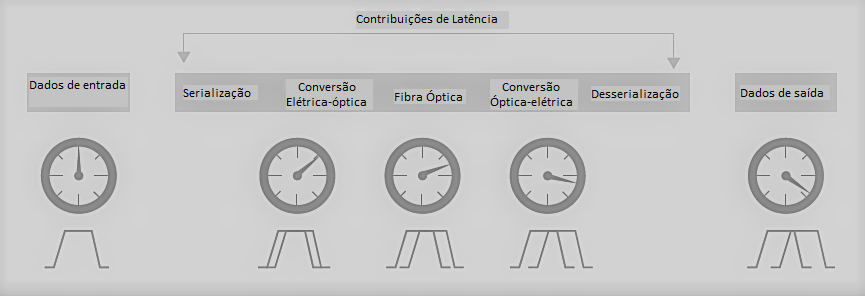
\includegraphics[width=12cm]{latency_link}
	\caption{Latência em comunicação entre dois pontos utilizando link óptico. Os principais pontos de inserção de latência na comunicação são resultantes dos processos de conversão elétrica-óptica, transmissão de dados, conversão óptica-elétrica e disponibilização dos dados no destino (desserialização e processamento). Adaptado de \cite{Art_Coffey}.}
	\label{fig_latency_link}
\end{figure}

Os pontos da rede de acionamento do chaveador óptico podem ser escolhidos em ramos de um grafo com muitos vértices (\emph{hops}) ou podem ser planejados para o estabelecimento de rotas específicas para comunicação com pontos críticos do sistema, estabelecendo um SLA (\emph{Service Level Agreement}) em camada físico.

Através da utilização do BSN é possível reduzir o grafo da rede possibilitando uma nova configuração de conexões e consequentemente uma nova variedade de rotas possíveis. Cada vez que o BSN ativa um \emph{bypass}, as duas arestas envolvidas são unificadas evitando o vértice das mesmas, criando assim um novo grafo com uma distância entre os dois vértices finais de um vértice a menos, como representado na Figura \ref{fig_bypass_exemplo}. Dessa forma, em caso de falha ou mudança de SLA, a topologia física pode ser alterada automaticamente.

Para isso certos cuidados devem ser tomados, como a utilização de chaveadores ópticos em pontos estratégicos da rede que não criem isolamento de equipamentos sem conexão. É importante também que os chaveadores utilizados possam ser controlados a partir do centro de controle da rede. Desta forma, em caso de alguma falha na rede pode-se reajustá-la de maneira automática garantindo a melhor operação em qualquer circunstância.

\begin{figure} % normalmente utilizar [!t]
	\centering
	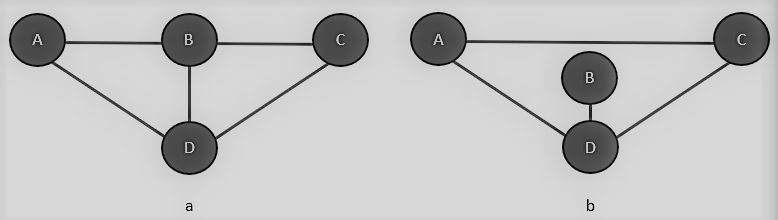
\includegraphics[width=10cm]{Bypass_exemplo_PB}
	\caption{Efeito da utilização do chaveador ótico. Em ``a'' pode-se ver a rede original contendo dois saltos entre os vértices A e C. Em ``b'' após o acionamento do dispositivo no vértice B pode-se ver e existência de apenas um salto entre os vértices A e C}
	\label{fig_bypass_exemplo}
\end{figure}

\section{Simulações}
\subsection{Cenário aplicável}
O BSN foi desenvolvido considerando-se aplicações como as descritas na Seção \ref{sec:Ambientacao}, ou seja, em cenários constituídos por redes representadas por grafos simples. É importante notar que este tipo de aplicação considera a existência de um vértice raiz, onde deve estar presente o centro de controle da rede. Dessa forma, todas as comunicações estabelecidas na rede devem ser originadas ou destinadas a este vértice.

Com o objetivo de avaliar o desempenho do BSN foram realizadas simulações considerando uma rede de testes fictícia representada pelo grafo da Figura \ref{fig_rede_estudo}. Neste grafo, consideraremos que o nó ``E'' é o nó raiz e os demais nós são equipamentos de campo com os quais precisam ser estabelecidas rotas de comunicação.

\begin{figure} % normalmente utilizar [!t]
	\centering
	\includegraphics[width=8.5cm]{Rede_Estudo_PB}
	\caption{Grafo da rede a ser avaliada.}
	\label{fig_rede_estudo}
\end{figure}

\subsection{Metodologia}
%Para a avaliação do desempenho do BSN foi utilizada a rede de estudos apresentada na Figura \ref{fig_rede_estudo}. Esta rede foi submetida a otimização através da utilização de protocolos conhecidos como o PRIM e o STP (\emph{Minimal Spanning Tree}) para comparação com o resultado obtido através do BSN.

Para comprovar a eficiência da proposta BSN foi realizada uma avaliação de desempenho comparando os protocolos já estabelecidos PRIM e STP com o BSN. A rede de testes utilizada foi representada na Figura \ref{fig_rede_estudo}.

\subsubsection{Restrições}
%O protocolo proposto foi desenvolvido para ser utilizado em redes ópticas de topologia \emph{mesh}. Para tanto, é necessário que a rede em questão possa ser representada por um grafo simples, ou seja, um grafo que não possui arestas paralelas ou pontas coincidentes (laços).

As simulações realizadas consideram apenas a topologia representada na Figura \ref{fig_rede_estudo}, cujas conexões foram inspiradas em uma rede SG real. Nesta rede as conexões entre os equipamentos são realizadas através de \emph{transceivers} bidirecionais que utilizam diferentes comprimentos de onda para TX e RX. Dessa forma a interconexão entre os equipamentos da rede deve respeitar a premissa de nunca ser realizada entre \emph{transceivers} de mesmo modelo visto que neste caso haveriam incompatibilidades entre os comprimentos de onda utilizados na transmissão e recepção de dados. Esta restrição, apesar de presente na rede estudada, não é um impeditivo para a utilização do BSN em outros tipos de redes ópticas, visto que existem diferentes modelos de chaveadores ópticos que podem adequar-se a tais redes.

%O conceito de funcionamento do BSN pode ser aplicado em redes metálicas caso seja utilizado um componente análogo ao chaveador óptico. Esta opção não foi abordada ou considerada no presente documento.
\subsection{Resultados Obtidos}
\label{sec:resultados}
\subsubsection{Avaliação do Protocolo \emph{Minimal Spanning Tree} - PRIM}
\label{sec:minimal_spanning_tree}
Para utilização do algoritmo PRIM, todas as arestas do grafo foram consideradas como possuindo o mesmo custo, representando uma rede sem o favorecimento de nenhuma rota em específico. A saída do algoritmo fornece uma nova configuração de grafo, baseada na original (grafo da Figura \ref{fig_rede_estudo}) e excluindo as arestas redundantes de maneira a obter o menor custo total. Ou seja, um grafo com todos os vértices conectados e o menor número de arestas possível.

Visto que este algoritmo busca a criação de um grafo com o menor número de arestas possível, ele não leva em consideração um vértice raiz, como é o caso desejado para a aplicação. Mas após a árvore geradora mínima resultante ser redesenhada considerando-se o vértice ``E'' como sendo o raiz obtém-se a rede apresentada na Figura \ref{fig_rede_otimizada_prim}.

\begin{figure} % normalmente utilizar [!t]
	\centering
	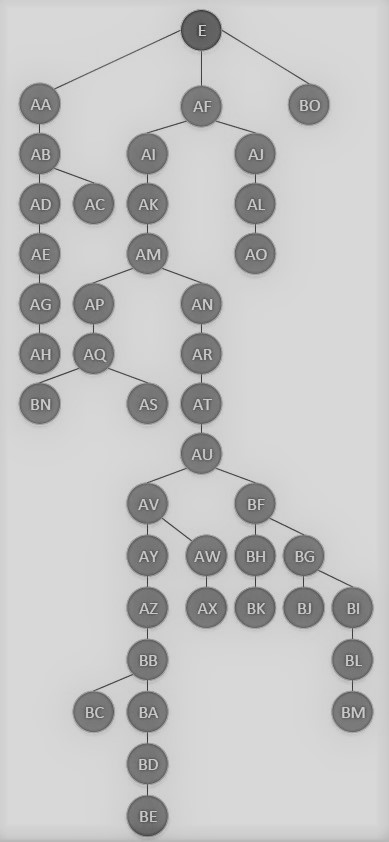
\includegraphics[width=4cm]{Otimizada_Prim_PB}
	\caption{Rede resultante após a utilização do algoritmo PRIM. O grafo representa a árvore mínima da rede e é possível notar que a profundidade máxima é de 15 saltos.}
	\label{fig_rede_otimizada_prim}
\end{figure}

\subsubsection{\emph{Spanning Tree Protocol} - STP}
A utilização do STP aplicado à rede de estudos apresentada na Figura \ref{fig_rede_estudo}, considerando o vértice ``E'' como sendo o vértice raiz, resulta no grafo de rede apresentado na Figura \ref{fig_rede_otimizada_STP}. Pode-se reparar que neste caso o STP calcula um grafo diferente do apresentado na Figura \ref{fig_rede_otimizada_prim} visto que o objetivo do protocolo não é calcular a rede com menor custo total mas sim a rede que apresente os menores custos possíveis entre o vértice raiz e os demais.

\begin{figure} % normalmente utilizar [!t]
	\centering
	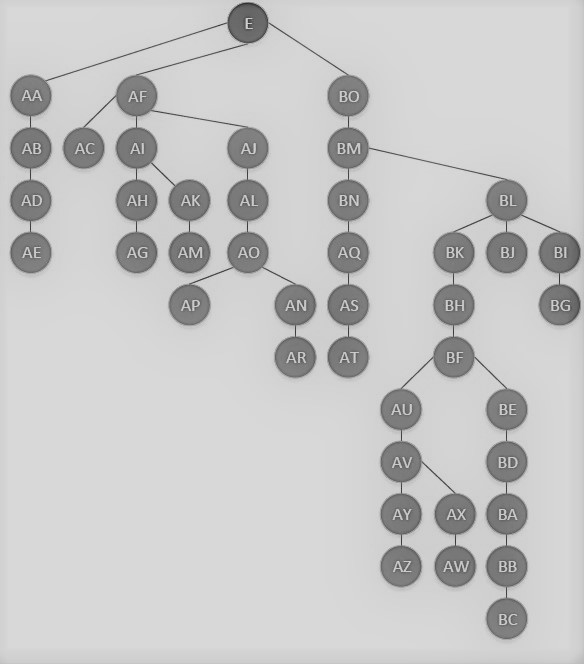
\includegraphics[width=6cm]{Otimizada_STP_PB}
	\caption{Rede resultante após a utilização do STP considerando o nó raiz como sendo o vértice ``E''. Percebe-se que a profundidade máxima da rede é de 11 saltos.}
	\label{fig_rede_otimizada_STP}
\end{figure}

\subsubsection{\emph{Bypass Seletivo de Nós} - BSN}
Utilizando o BSN aplicado à mesma rede de estudos utilizada nas outras simulações e também considerando o vértice ``E'' como sendo o vértice raiz do grafo obtém-se o resultado apresentado na Figura \ref{fig_rede_otimizada_BSN}.

\begin{figure} % normalmente utilizar [!t]
	\centering
	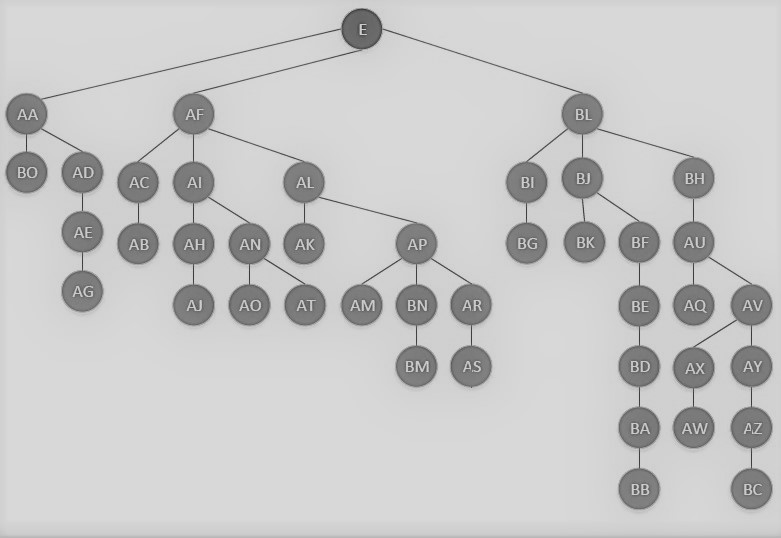
\includegraphics[width=8cm]{Otimizada_BSN_PB}
	\caption{Rede resultante após a utilização do BSN. Percebe-se que a profundidade máxima da rede é de 7 saltos.}
	\label{fig_rede_otimizada_BSN}
\end{figure}



\subsection{Discussões e Análise dos Dados}

O objetivo principal do BSN é o de fornecer configurações de topologia de rede ópticas que possibilitem o estabelecimento de comunicações com valores de latência otimizados. Como descrito na seção \ref{sec:proposta} do presente documento, cada equipamento existente em um ramo de comunicação é uma fonte de inserção de latência na rede, sendo assim pode-se afirmar que cada \emph{hop} adicional em um ramo do grafo resultante da rede pode ser traduzido como uma inserção de latência no mesmo. Logo, ao encurtar os ramos do grafo minimiza-se o valor de latência da rede.

A partir dos resultados apresentados na Seção \ref{sec:resultados} pode-se notar uma sensível mudança no parâmetro de profundidade máxima do grafo entre os métodos utilizados, o que é possível observar através de uma análise comparativa entre as Figuras \ref{fig_rede_otimizada_prim}, \ref{fig_rede_otimizada_STP} e \ref{fig_rede_otimizada_BSN} onde nota-se uma variação na largura do mesmo em relação a profundidade. Ou seja, temos um grafo com uma média de \emph{hops} menor para cada destino, resultando desta forma em menores valores de latência para a rede como um todo.

A Tabela \ref{tab_comparacao} é o resultado da compilação dos resultados apresentados na seção \ref{sec:resultados}.

\begin{table}[ht]
\renewcommand{\arraystretch}{1.4}
\centering
\caption{Comparação entre as topologias de rede otimizadas por cada um dos protocolos.}
\label{tab_comparacao}
\begin{tabular}{|c|c|c|}
\hline
\multicolumn{1}{|c|}{Protocolo} & \begin{tabular}[c]{@{}c@{}}Chaves ópticas\\ utilizadas\end{tabular} & \begin{tabular}[c]{@{}c@{}}Profundidade \\ da Rede\end{tabular} \\ \hline
PRIM & 0 & 15 \\ \hline
STP & 0 & 11 \\ \hline
BSN & 15 & 7 \\ \hline
\end{tabular}
\end{table}

Através da análise da Tabela \ref{tab_comparacao} pode-se notar expressiva melhora na redução do diâmetro da rede ao utilizar o BSN. 

%A Tabela \ref{tab_percentual} mostra o percentual de melhoria nos parâmetros avaliados entre os três protocolos considerando a árvore geradora mínima do grafo (\emph{Minimal Spanning Tree} - PRIM) como base.

Para comparação do percentual de melhoria entre as redes, é necessário considerar o conceito de Latência Sistêmica, definida como a soma dos atrasos decorrentes da transmissão e conversão dos dados, e convenientemente ilustrada na Figura \ref{fig_latencia_sistemica}. A latência de conversão é específica à aplicação e ao equipamento ativo envolvido, ou seja, depende da capacidade de processamento do equipamento; a latência de transmissão por sua vez depende da distância em que o enlace é estabelecido e do meio que está sendo utilizado. De maneira geral, a latência de transmissão em fibras ópticas é muitas ordens de grandeza menor que a de conversão e por isso é frequentemente desprezada.

\begin{figure} % normalmente utilizar [!t]
	\centering
	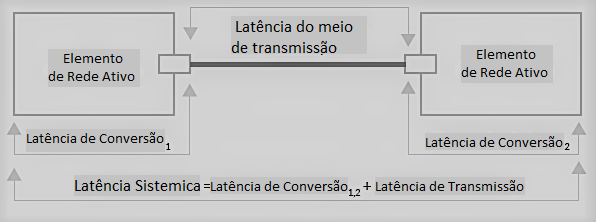
\includegraphics[width=9cm]{latency_systemic_PB}
	\caption{Latência sistêmica. Percebe-se que trata-se de um fenômeno cumulativo e qualquer \emph{delay} introduzido pelo meio de transmissão ou qualquer equipamento ativo contribui para o aumento do seu valor. Adaptado de \cite{Art_Coffey}.}
	\label{fig_latencia_sistemica}
\end{figure}

Para fins de comparação pode-se analisar a latência de transmissão considerando o meio fibra-óptica através da velocidade média de propagação da luz no núcleo da fibra, de onde pode-se tirar que a latência neste meio é de aproximadamente 5 \textmu s/km. Logo, considerando que cada enlace entre dois pontos na rede da Figura \ref{fig_rede_estudo} possua, em média, 1km de extensão e que o tempo de processamento em cada um dos nós (desconsiderando o aumento de tempo no caso de excesso de processamento em determinados nós) é de 1ms na média (já incluindo os tempos das conversões de meio necessárias), gera-se a Tabela \ref{tab_percentual} que mostra a melhoria nos parâmetros avaliados entre os três protocolos.

A Figura \ref{fig_tab_percentual} relaciona alguns dos parâmetros mostrados na Tabela \ref{tab_percentual}. Nesta figura fica claro a relação de melhoria do protocolo proposto, quando aplicados à rede estudada, em comparação com os demais. É interessante salientar que, mesmo em redes relativamente pequenas como no caso apresentado (apenas 47 pontos de automação), a utilização do BSN forneceu uma redução de mais de 33\% de latência máxima, valor muito expressivo para a aplicação em questão. Espera-se que a melhoria seja ainda maior em redes com mais nós, haja vista a maior possibilidade de reconfiguração da rede. 

\begin{table}[ht]
\renewcommand{\arraystretch}{1.4}
\centering
\caption{Tabela comparativa de melhoria de parâmetros entre os três protocolos avaliados.}
\label{tab_percentual}
\begin{tabular}{|l|c|c|c|c|c|}
\hline
\multicolumn{1}{|c|}{} & PRIM & STP & BSN & \begin{tabular}[c]{@{}c@{}}\% de melhoria\\ BSN vs PRIM\end{tabular} & \begin{tabular}[c]{@{}c@{}}\% de melhoria\\ BSN vs STP\end{tabular} \\ \hline
\begin{tabular}[c]{@{}l@{}}Profundidade\\ da Rede\end{tabular} & 15 & 11 & 7 & 53,33\% & 36,36\% \\ \hline
\begin{tabular}[c]{@{}l@{}}Latência Máxima\footnotemark\\ {[}ms{]}\end{tabular} & 16,075 & 12,055 & 8,035 & 50\% & 33,35\% \\ \hline
\begin{tabular}[c]{@{}l@{}}Latência Total\footnotemark\\ {[}ms{]}\end{tabular} & 342,5 & 246,02 & 187,73 & 45,19\% & 23,69\% \\ \hline
\end{tabular}
\end{table}
\footnotetext[1]{Calculada como sendo a latência existente no ramo mais comprido do grafo.}
\footnotetext[2]{Calculada como sendo a soma de todas as latências de todos os enlaces do grafo.}

\begin{figure} % normalmente utilizar [!t]
	\centering
	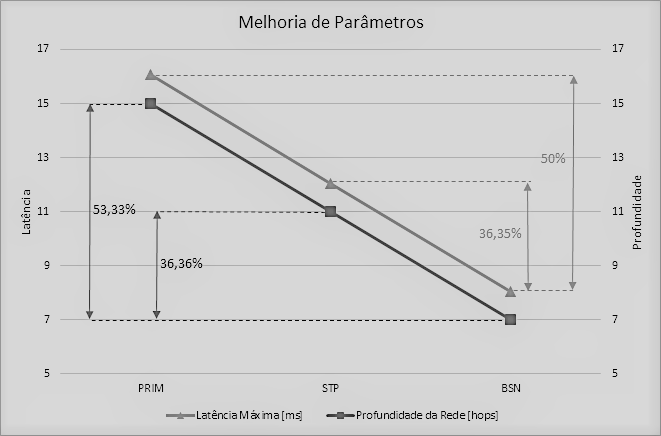
\includegraphics[width=9cm]{Tabela2GraficoPB}
	\caption{Comparação entre parâmetros resultantes após a utilização dos protocolos utilizados na otimização da rede estudada. Esperam-se resultados ainda melhores em redes \emph{Mesh} com mais nós.}
	\label{fig_tab_percentual}
\end{figure}

\section{Conclusão}

%As redes \emph{Smart Grid} estão se tornando realidade devido a diversos fatores, dentre os quais pode-se salientar a utilização de fontes renováveis de energia e a massiva utilização de sensores e atuadores esperados para um futuro próximo. Devido à grande variedade de requisitos de rede necessários para atender as demandas presentes e futuras deste tipo de rede, espera-se que a infraestrutura utilizada para comunicação seja segura, eficiente, rápida e altamente disponível.
%
%Estas necessidades justificam facilmente a utilização de tecnologias como a fibra óptica e topologias como a \emph{mesh} para o estabelecimento da infraestrutura de comunicação a ser utilizada. Neste sentido é necessário atentar à possíveis inserções de latência devido às características fundamentais deste tipo de topologia.
Este trabalho teve como objetivo tratar de possíveis inserções de latência em redes ópticas \emph{mesh} devido às características fundamentais deste tipo de topologia, que conforme visto, deve atender aos requisitos demandados pelo \emph{Smart Grid}.

Através da comparação entre os resultados apresentados, com e sem a utilização do método proposto, fica fácil perceber que a utilização das chaves ópticas foi capaz de minimizar a latência de uma rede já otimizada através da utilização de um protocolo de rede padrão como o STP. Isto deve-se ao fato da manipulação do grafo da rede ter sido realizada em camada 1. Dessa forma torna-se possível o estabelecimento de políticas de SLA em nível físico, ou seja, sem nenhum tipo de processamento direto no encaminhamento dos pacotes, o que sem dúvida é um ponto de grande avanço quando comparado com técnicas comuns de priorização de serviço.

No exemplo utilizado pode-se perceber uma melhora significativa no número de saltos necessários para a realização da comunicação. Acredita-se que valores ainda mais significativos sejam obtidos em redes maiores devido a maior combinação de possibilidades para utilização dos chaveadores ópticos.

Sendo assim, o BSN cumpre seu principal objetivo oferecendo uma maneira eficaz de diminuição de latência em redes ópticas de topologia \emph{mesh} independentemente do protocolo de busca de rotas utilizado. 


%\section{References}


\bibliographystyle{sbc}
\bibliography{IEEEabrv,SMMC2018}
\end{document}
